\section{Klassifizierung}
\label{Klassifizierung}
Die Aufgabe der Klassifikation "ubernimmt in dieser Arbeit ein k"unstliches Neuronales Netz (KNN). KNNs sind in Struktur und Arbeitsweise vom menschlichen Nervensystem inspiriert \cite{kruse2011computational} und versuchen intelligente Entscheidungen zu treffen. Zun"achst wurde nur ein einzelnes Perzeptron verwendet, welches eine Nervenzelle simulieren sollte. Das Perzeptron besitzt einen oder mehrere Eing"ange, an die unterschiedlich gewichtete Signale angelegt werden, und mindestens einen Ausgang, der aktiv wird, falls der interne Schwellwert "uberschritten wird. Dies ist stark an die Natur angelehnt, die Eing"ange entsprechen den Dendriten einer Nervenzelle und die Ausg"ange den Endkn"opfchen\cite{kruse2011computational}. \\
Ein einzelnes Perzeptron ist aber in seiner M"achtigkeit sehr eingeschr"ankt, da es nur linear separierbare Funktionen korrekt darstellen kann. Dieses Problem l"ost die Zusammenfassung mehrerer Perzeptren zu einem Netz, solche Netze zu trainieren wurde aber erst durch den von \cite{werbos1974beyond} beschriebenen error-backpropagation Algorithmus m"oglich. Seitdem wurden verschiedene Typen von Netzen und Formen von Perzeptren entwickelt, um unterschiedlichen Aufgaben gerecht zu werden. Diese Arbeit verwendet ein mehrschichtiges Perzeptron (Multilayer Perceptron MLP) in einem vorw"arts gerichteten Netz (feed forward), dabei werden f"ur die Klassifikation sigmoide Aktivierungsfunktionen verwendet. Die verwendeten Technologien werden in \ref{Stand der Technik} genauer beschrieben.


\subsection{Weka}
\label{Weka}
Weka ist ein bekanntes Framework f"ur maschinelles Lernen. Die in Java geschriebene Software wurde von der \textit{University of Waikato, New Zealand} entwickelt und unter \textit{GNU General Public License} ver"offentlicht\cite{WekaHaupt}. \\
Weka bietet viele, f"ur diese Arbeit wichtige Funktionen an. Insbesondere die integrierten Filter und die automatische Interpretation von Instanzen zur Klassifikation ersparen viel Arbeit. Weka implementiert eine Vielzahl von Klassifikatoren, darunter auch das Multilayer Perceptron (MLP).
Au{\ss}erdem bietet es einige Methoden zur Evaluation der erstellten Modelle, wie zum Beispiel die k-fold-Evaluierung. Dabei ist es jedoch nicht auf die massiv parallele Verarbeitung moderner Prozessoren ausgelegt und skaliert nicht horizontal.\\
In dieser Arbeit wird Wekas Implementierung des MLP benutzt. Der Algorithmus bietet sich wegen der einfachen Verwendung bei gleichzeitiger M"oglichkeit zu parametrieren an. Die bereits implementierten  Funktionen zur Filterung und Evaluation verringern den Implementierungsaufwand f"ur die hier erstellte Software.

\subsection{Stand der Technik}
\label{Stand der Technik}
\cite{liang2010load} und \cite{srinivasan2006neural} legen die Verwendung von MLPs gegen"uber Radiale-Basisfunktionen-Netzen (Radial Basefunction Net RBF) nahe, da sie mit diesen deutlich bessere Ergebnisse erzielen. 
Bei einem MLP handelt es sich um ein streng geschichtetes KNN. Das bedeutet, dass keine Verbindungen innerhalb der Schichten bestehen und die Eing"ange einer Schicht nur mit den Ausg"angen der vorherigen Schicht verbunden sind \cite{kruse2011computational}, siehe dazu auch Abbildung~\ref{mlp}. Ein MLP besteht immer aus mindestens zwei Schichten, n"amlich der Eingabe- und der Ausgabeschicht, die Anzahl der versteckten Schichten dazwischen ist beliebig.\\
Die in Abbildung~\ref{sinus} gezeigte Aktivierungsfunktion ist beispielhaft f"ur die Aktivierung der Ausg"ange eines Perzeptrons im Netz, die Eingaben werden mit ihren jeweiligen Gewichten multipliziert und anschlie{\ss}end addiert, ist der resultierende Wert gr"o{\ss}er als der Schwellwert $\Theta$ wird der Ausgang aktiv. Die Nutzung der Sinus-Funktion f"uhrt hierbei jedoch dazu, dass es keinen Sprung von 0 auf 1 gibt, sondern einen stetigen Anstieg. F"ur das Training mit dem error-backpropagation Algorithmus ist jedoch die Differenzierbarkeit notwendig, welche die Sprungfunktion nicht besitzt \cite{kruse2011computational}. \\
Der error-backpropagation Algorithmus berechnet den Fehler zwischen gew"unschter und tats"achlicher Ausgabe des Netzes im Training und gibt anschlie{\ss}end das Fehlersignal r"uckw"arts durch das Netz, dabei passen die Perzeptren die Eingabegewichte an, um den Fehler zu minimieren \cite{kruse2011computational}. So wird der Trainingsdatensatz mehrfach durchlaufen und der Fehler immer weiter verringert, ma{\ss}gebender Faktor f"ur die Verringerung des Fehlers ist die Lernrate. Sie gibt an, wie stark die Gewichte in jedem Schritt angepasst werden.  Eine h"ohere Lernrate f"uhrt dazu, dass das Netz schneller in Richtung des lokalen Minimums konvergiert, kann aber auch dazu f"uhren, dass es das Minimum "uberspringt und es nie genau erreicht. Dies kann aber durchaus erw"unscht sein, wenn durch die hohe Konvergenzgeschwindigkeit nicht optimale Minima "ubersprungen werden. Au{\ss}erdem ben"otigt eine niedrige Lernrate im Allgemeinen mehr Epochen, um das lokale Minimum zu erreichen. Die Anzahl der Epochen gibt dabei an, wie oft das Netz die Trainingsinstanzen w"ahrend des Trainings durchl"auft. Ist die Anzahl der Epochen zu gering, kann der Fehler nicht ausreichend minimiert werden. Siehe dazu in Abbildung~\ref{momentum} das Beispiel auf der linken Seite, 11 Perioden reichen hier nicht, um das Minimum zu erreichen. 
Zus"atzlich verwenden wir das Momentterm-Verfahren aus \cite{rumelhart1988learning}, welches die Lernrate erh"oht, solange sich der Fehler verringert und die Lernrate gemindert wenn der Algorithmus um ein Minimum oszilliert und sich der Fehler nicht mehr verringert. Das Momentum ist hilfreich, um den Trade-off zwischen Laufzeit des Trainings und G"ute des Ergebnisses zu verbessern. Eine niedrige Lernrate verbessert im Allgemeinen die Ann"aherung an das lokale Minimum, verl"angert aber auch die Trainingszeit, weil sie mehr Schritte zur ausreichenden Minimierung des Fehlers ben"otigt. Durch die Erh"ohung und Verringerung der Lernrate kann das Momentum helfen eine gute L"osung in weniger Epochen zu erzielen. Dies garantiert jedoch nicht, dass das globale Minimum f"ur den gemachten Fehler gefunden wird. \\
\cite{pinkus1999approximation} zeigt, dass man jede stetige Funktion mit einem MLP mit nur einer versteckten Schicht mit beliebig geringem Fehler approximieren kann. Das bedeutet aber nur, dass eine Netzstruktur gefunden werden kann, mit der jede beliebige Fehlerschranke unterschritten wird. Laut \cite{kruse2011computational} ist es aber in der Praxis h"aufig von Vorteil mehrere versteckte Schichten einzubauen um schneller an eine gute Approximation zu kommen. \\
Die Ausgabeschicht wird im 1-zu-n Schema modelliert. Das bedeutet, dass die sechs Klassen durch sechs Knoten in der Ausgabeschicht modelliert werden, als Ausgabe wird dann der Knoten mit der h"ochsten Ausgabe gew"ahlt. Im Optimalfall hat einer der sechs Knoten als Ausgabe den Wert 1 und die anderen Knoten den Wert 0, durch die Verwendung der Sinus-Funktion ist dies jedoch nicht immer der Fall. 

\begin{figure}[h]
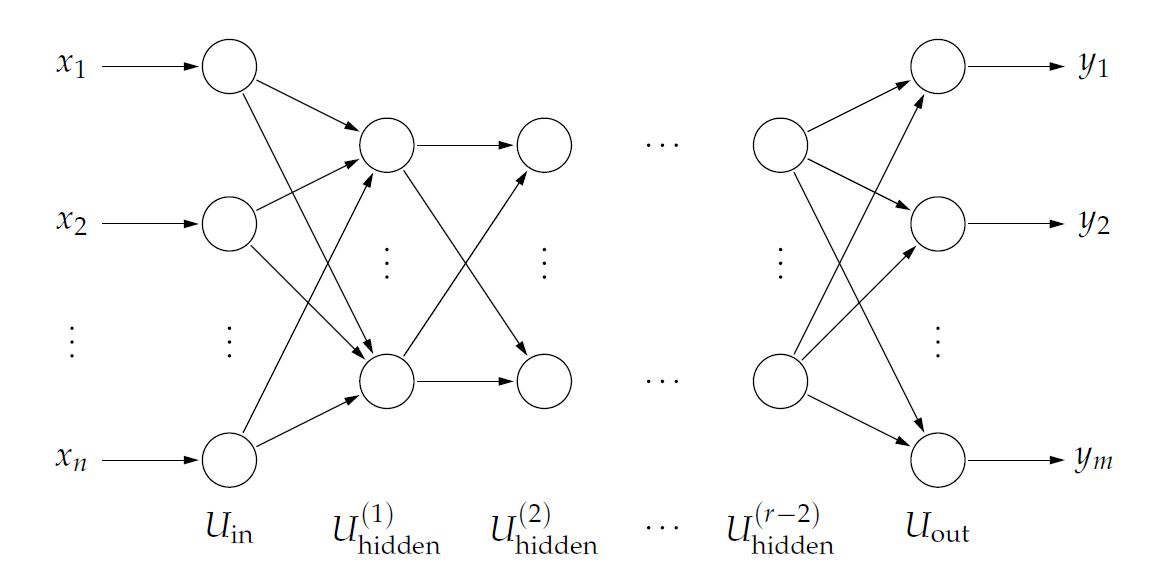
\includegraphics[width=\textwidth]{1_Grafiken/fig1kruse.jpg}
	\caption[Allgemeiner Aufbau eines mehrschichtigen Perzeptrons]{Grafik zum allgemeinen Aufbau eines aus r Schichten bestehenden MLPs aus \cite{kruse2011computational}, $x_a$ bezeichnen die Eingaben, $y_b$ die Ausgaben und $U_c$ die verschiedenen Schichten des Netzes}
\label{mlp}
\end{figure}

\begin{figure}[h]
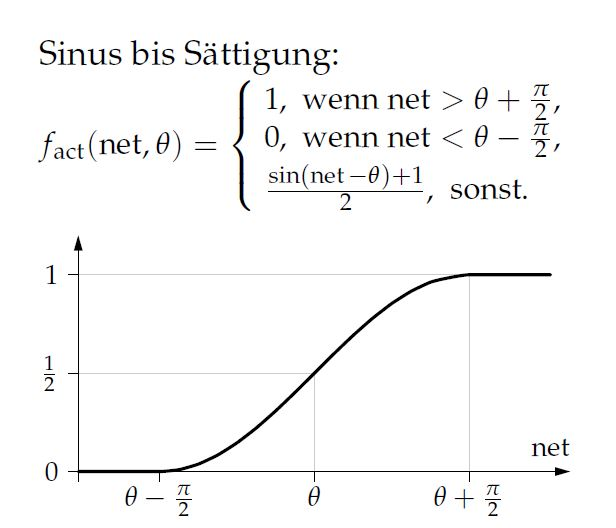
\includegraphics[width=0.6\textwidth]{1_Grafiken/fig2kruse.jpg}
	\caption[Beispiel einer Aktivierungsfunktion]{Beispiel einer Aktivierungsfunktion aus \cite{kruse2011computational}, $\Theta$ ist der Schwellwert f"ur die Aktivierung des Ausgangs und net die Eingaben multipliziert mit den Eingabegewichten}
\label{sinus}
\end{figure}

\begin{figure}[h]
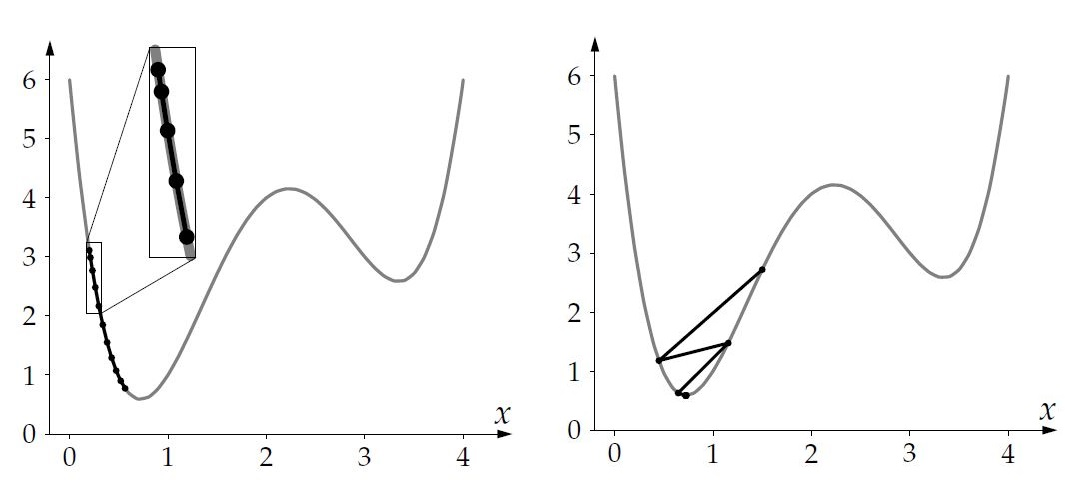
\includegraphics[width=\textwidth]{1_Grafiken/fig3kruse.jpg}
	\caption[Beispiel f"ur Momentterm-Verfahren]{Beispiel Momentterm-Verfahren aus \cite{kruse2011computational}, links sieht man die Erh"ohung einer f"ur den Abschnitt zu niedrig gew"ahlten Lernrate, rechts die Verringerung der Lernrate wegen Oszillationen}
\label{momentum}
\end{figure}


\subsection{Parameter}
\label{Parameter}
Ein MLP hat einige wichtige Parameter, die zur Genauigkeit der Klassifikation beitragen. Dieses Kapitel soll aber lediglich auf die Parameter und die von der Weka Dokumentation \cite{WekaMLP}
empfohlenen Wertebereiche für diese hinweisen. Die besten Werte f"ur jeden Parameter werden in Kapitel~\ref{Evaluation} ermittelt. Mit dem ersten wichtigen Parameter hat sich bereits das vorherige Kapitel besch"aftigt: Die Features. Diese spielen in der Klassifikation eine zentrale Rolle und wurden daher gesondert behandelt.\\
Die Epochen $N$ geben die Anzahl der Iterationen des error-backpropagation Algorithmus an, sie sollten ausreichend groß gewählt werden, ein größeres $N$ erhöht aber auch die nötige Zeit zum erstellen des Modells. Als Standardwert gibt Weka eine Epochenanzahl von 500 an.\\ 
Die Geschwindigkeit, mit der die Gewichte innerhalb des Netzes angepasst und somit der Fehler minimiert wird, wird durch die Lernrate $L$ bestimmt. Die Dokumentation empfiehlt eine Lernrate zwischen 0 und 1, als Standardwert wird 0,3 verwendet.\\
Das Momentum $M$ verändert die Lernrate zwischen den Iterationen, der Wert vom $M$ gibt an, wie stark $L$ innerhalb eines Schritts verändert werden kann. Empfohlen sind Werte zwischen 0 und 1, Standardwert ist 0,2.\\
Auch die Struktur des Netzes $H$ kann einen positiven Einfluss auf die Klassifikation haben. Dabei ist die Anzahl der Knoten in  Eingabe- und Ausgabeschicht (Input-/Outputlayer) festgeschrieben, die Eingabeschicht hat so viele Knoten wie es Features gibt und die Ausgabeschicht so viele Knoten wie es Klassen gibt. Die versteckten Schichten (Hiddenlayer) dazwischen sind aber variabel, hier wird von Weka standardmäßig eine Schicht vorgegeben, diese hat als Knotenanzahl den Durchschnitt der Knotenanzahl von  Eingabe- und Ausgabeschicht. Hier kann die Veränderung der Knotenanzahl und das Hinzuf"ugen weiterer versteckter Schichten getestet werden \cite{kruse2011computational}.\\
